\chapter{Herramientas utilizadas}
\label{cap:capitulo3}

El desarrollo de los 2 nuevos ejercicios de Robotics Academy han abarcado varios campos: programación, Docker, modelado y simulación de robots, ROS y ROS2, visión artificial, machine learning, desarrollo web... por lo que es necesario introducir y describir las herramientas y tecnologías utilizadas.




% -- SECCIÓN C++
% ----------------
\section{C++}
\label{sec:c++}

C++ es un lenguaje de programación diseñado en 1979 por Bjarne Stroustrup. Deriva del lenguaje C, y destaca principalmente porque incorpora el paradigma de la Programación Orientada a Objetos (POO). Además, incorpora una gran cantidad de nuevas librerías para facilitar la programación como por ejemplo las librerías estandar y STL (Standard Template Library).\\

\begin{code}[H]
\begin{lstlisting}[language=C++]
#include <iostream>

int main(int argc, char ** argv)
{
	std::cout << "Hello World!\n";
	return 0;
}
\end{lstlisting}
\caption[Hola mundo en C++]{Hola mundo en C++}
\label{cod:holamundo_cplusplus}
\end{code}

\textbf{¿Cuál ha sido la utilidad de C++ en este proyecto?} La programación de un \textbf{plugin} \footnote{\textbf{Plugin}: Complemento que añade una funcionalidad extra o mejora a un programa} que permite mover a una persona simulada en Gazebo \footnote{\textbf{Gazebo}: simulador robótico} con el teclado.\\




% -- SECCIÓN PYTHON
% -------------------
\section{Python}
\label{sec:python}

Python es un lenguaje de programación interpretado \footnote{\textbf{Interprete} (programación): programa informático que se encarga de ejecutar las instrucciones de otro programa sin compilación previa} que destaca por su legibilidad, facilidad y soportabilidad a la programación Orientada a Objetos. Posee características particulares que lo diferencian de otros lenguajes de programación como puede ser el uso estricto de indentación en bloques de código.\\

\begin{code}[H]
\begin{lstlisting}[language=Python]
print("Hola mundo")
\end{lstlisting}
\caption[Hola mundo en Python]{Hola mundo en Python}
\label{cod:holamundo_python}
\end{code}

\textbf{¿Cuál ha sido la utilidad de Python en este proyecto?} El desarrollo de la infraestructura interna que da soporte a los dos nuevos ejercicios de Robotics Academy, programación de nodos de ROS (más en la sección \ref{sec:ros}) y ficheros de lanzamiento, creación de los módulos HAL y GUI y desarollo de la solución a los ejercicios.\\




% -- SECCION ROS
% ----------------
\section{ROS (Robot Operating System)}
\label{sec:ros}
ROS (Robot Operating System) es un middleware \footnote{\textbf{Middleware}: software que se sitúa entre las aplicaciones y el sistema operativo} que ayuda a la programación de robots a través de varias librerías y herramientas desarrolladas por la comunidad de software libre. Entre las ayudas que proporciona este framework están la abstracción del hardware, controladores de dispositivos, herramientas de visualización y geometría espacial entre otros.\\

Desde un principio, ROS se ha ejecutado sobre sistemas operativos de tipo Unix (Ubuntu - principal), aunque han ido surgiendo versiones beta para otros sistemas como Windows o MacOS X. La primera distribución de ROS salió en 2010 (ROS Box Turtle) y a partir de ahí han ido surgiendo nuevas distribuciones siendo la actual y estable ROS Noetic.\\

El funcionamiento de ROS se basa en una arquitectura cliente-servidor centralizado donde un nodo principal se encarga del intercambio de mensajes entre otros nodos que forman la aplicación (remotos o locales), los cuales se comportan como publicadores o suscriptores del proceso de comunicación. El objetivo es dividir el software robótico en secciones o nodos que se encargan de realizar tareas específicas de manera paralela: recogida de datos de la cámara, ejecución de una máquina de estados o árboles de comportamiento (Behavior Trees), recogida de las lecturas del láser, navegación, etc.\\

El intercambio de mensajes se realiza a través \textbf{topics}. Un nodo puede tener \textbf{publicadores}, \textbf{suscriptores} o ambos. Cuando un nodo publica un mensaje lo hace a través de un topic que gestiona el nodo maestro. Si otro nodo quiere leer ese mensaje tendrá que suscribirse al tópic correspondiente. Por ejemplo: en nuestro robot Turtlebot2 podemos comandar velocidades enviando mensajes de tipo \textbf{geometry\_msgs.msg.Twist} a través del topic \textbf{/cmd\_vel}. En la figura se puede ver con más detalle \ref{fig:ros_master_comunicacion}\\

\begin{figure} [H]
  \begin{center}
    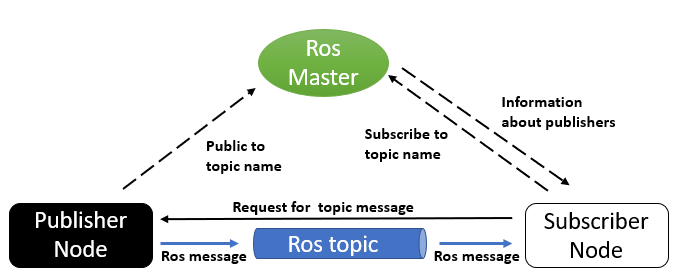
\includegraphics[width=15cm]{imagenes/ros_master_communication.png}
  \end{center}
  \caption{Comunicación del nodo Master con los nodos Intermedios (ROS)}
  \label{fig:ros_master_comunicación}
\end{figure}\

ROS incorpora un conjunto de librerías para ser usadas en C++ y Python. Con estos lenguajes de programación podemos desarrollar los nodos de los paquetes que tendrá nuestra aplicación. También incorpora un conjunto de comandos de \textbf{Shell} (términal) para hacer tareas de depuración, creación, compilación, etc.\\

En 2016 surge ROS 2, nuevo framework basado en ROS con muchas más mejoras como la \textbf{calidad de servicio}, los \textbf{lifecycle nodes} o \textbf{seguridad} (DDS) para asegurar la autenticación de los nodos y la integridad de los mensajes. Al igual que con ROS 1 ha tenido varias distribuciones siendo la primera \textbf{ROS Ardent}. La versión más reciente y estable es \textbf{ROS Foxy}, que es la que hemos usado en este proyecto.\\

Aprender ROS no es una tarea sencilla y requiere mucha dedicación y esfuerzo. Por lo tanto, el objetivo de Robotics Academy es proporcionar una interfaz de programación sencilla para programar robots sin necesidad de saber ROS. Es decir, el usuario tiene acceso a unas librerías HAL y GUI, las cuales usan por debajo nodos de ROS.\\

\textbf{¿Cuál ha sido la utilidad de ROS2 en este proyecto?} Crear los ficheros \textbf{interfaces} (laser.py, motors.py, camera.py, ...) que se comunican con los topics necesarios para el control del robot Turtlebot 2.\\




% -- SECCION URDF
% -----------------
\section{URDF}
\label{sec:urdf}

\textbf{URDF (United Robotics Description Format)} es un lenguaje de marcado para describir robots (eslabones, uniones, jerarquías, modelo visual, modelo de collisión, modelo inercial, controladores, etc) que usa la gramática de XML. Se utiliza tanto para robots reales como simulados.\\

Por lo general el robot se divide en su mayoría en eslabones (links) y uniones entre eslabones (joints), de manera que se forma un árbol jerárquico desde un eslabón principal (root) hasta los eslabones terminales.\\

Para definir un link hay que proporcionar un modelo visual, un modelo de colisión y un modelo inercial. Después se define el joint que une el eslabón que hemos definido con otro mediante una jerarquía de padres e hijos. En el siguiente código podemos ver un ejemplo de como se definiría un cubo de 1 metro por lado para su representación en un simulador.\\

\begin{code}[H]
\begin{lstlisting}
<?xml version="1.0"?>
<robot name="simple_cube">
	<link name="base_link">
		<visual>
			<origin xyz="0 0 0"/>
			<geometry>
				<box size="1.0 1.0 1.0"/>
			</geometry>
		</visual>
		<collision>
			<origin xyz="0 0 0"/>
			<geometry>
				<box size="1.0 1.0 1.0"/>
			</geometry>
		</collosion>
		<inertial>
			<origin xyz="0 0 0" /> 
			<mass value="1.0" />
			<inertia  ixx="1.0" ixy="0.0"  ixz="0.0"  iyy="1.0"  iyz="0.0"  izz="1.0"/>
		</inertial>
	</link>
</robot>
\end{lstlisting}
\caption[Ejemplo de código URDF: Definición de un cubo]{Ejemplo de código URDF: Definición de un cubo}
\label{cod:codigo_urdf}
\end{code}

\textbf{¿Cuál ha sido la utilidad de URDF en este proyecto?} Para la creación del modelo Turtlebot 2 simulado en ROS Foxy.
\begin{figure} [H]
  \begin{center}
    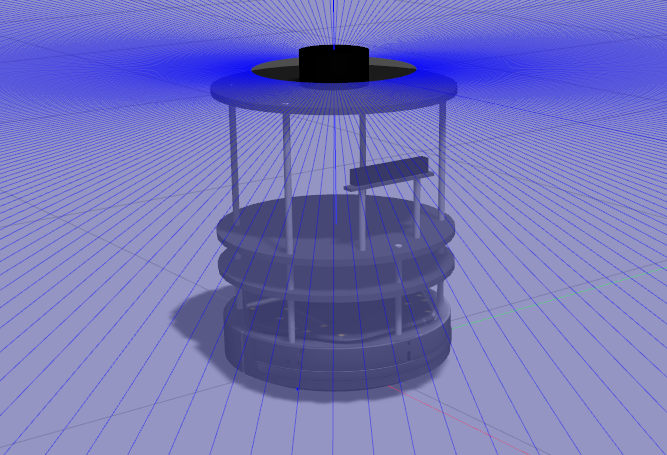
\includegraphics[width=10cm]{imagenes/turtlebot2-sim.png}
  \end{center}
  \caption{Modelo Turtlebot2 simulado (definido mediante URDF)}
  \label{fig:ros_master_comunicación}
\end{figure}\




% -- SECCION XACRO
% ------------------
\section{XACRO}
\label{sec:xacro}

XACRO (XML Macros) es un lenguaje XML diseñado para crear macros \footnote{\textbf{macro}: plantilla que define un patrón} en URDF. Con XACRO conseguimos diseños URDF mucho más legibles y sencillos. De esta manera podemos estructurar el diseño de un robot en componentes más pequeños y repetitivos. Por ejemplo: para el diseño del robot Turtlebot2 creamos una macro que se pueda aplicar a todos las barras verticales que sujetan la estructura del robot.\\

Una vez que tenemos nuestro diseño en XACRO, podemos exportarlo a URDF mediante el paquete de ROS denominado \textbf{xacro}. Su comportamiento es semejante al preprocesador de los lengauejes de programación como C: la macro la sustituye por el código URDF deseado teniendo en cuenta el valor de la variables que haya definido el programador.\\

\textbf{¿Cuál ha sido la utilidad de XACRO en este proyecto?} Diseñar un diseño sencillo y flexible del robot Turtlebot2. En el capítulo \ref{cap:capitulo4} describiremos mejor los detalles mediante algunas muestras del diseño.\\




% -- SECCION HTML Y CSS
% -----------------------
\section{HTML y CSS}
\label{sec:html_css}

\textbf{HTML (HiperText Markup Language)} es un lenguaje de marcado de tipo XML para el diseño de la estructura de las páginas web. Es un lenguaje que entiende el navegador web y se suele acompañar mediante una hoja de estilos que nos proporciona el lenguaje \textbf{CSS (Cascading Style Sheets)} para crear el estilo gráfico de la página web.\\


\begin{code}[H]
\begin{lstlisting}
<p>Esto es un parrafo en HTML</p>
\end{lstlisting}
\begin{lstlisting}
p {
	background-color: #FF0000;
}
\end{lstlisting}
\caption[Ejemplo de HTML y CSS]{Ejemplo de HTML y CSS: Todos los párrafos tienen el fondo rojo}
\label{cod:codigo_urdf}
\end{code}

\textbf{¿Cuál ha sido la utilidad de HTML y CSS en este proyecto?} Diseñar y dar estilo a la plantilla web de los 2 nuevos ejercicios de Robotics Academy. El diseño se base en seguir las plantillas de los demás ejercicios con algunos pequeños cambios e incorporaciones específicos.\\




% -- SECCION JAVASCRIPT
% -----------------------
\section{Javascript}
\label{sec:javascript}

\textbf{Javascript} es un lenguaje de programación interpretado que destaca por ser utilizado en el lado del cliente, en el Frontend de una página web que lee el navegador. Con Javascript podemos crear páginas web dinámicas a través de la definición de eventos que provocan resultados en el Backend (si tiene) o en la propia estructura HTML. Javascript puede usarse para multitud de tareas: Websockets, juegos, animaciones, etc.\\

\textbf{¿Cuál ha sido la utilidad de Javascript en este proyecto?}
En las plantillas web de Robotics Academy se usa Javascript para comunicar los eventos de la página con el fichero maestro de cada ejercicio que se llama \textbf{exercise.py}.\\




% -- SECCIÓN DOCKER
% -------------------
\section{Docker}
\label{sec:docker}

\textbf{Docker} es un framework que nos permite desplegar aplicaciones dentro de contenedores software que pueden ejecutar sobre cualquier sistema operativo.\\

La creación de imágenes se realiza mediante ficheros \textbf{Dockerfile} donde el programador indica los comandos (de Unix) necesarios para la construcción y despliegue de su aplicación.\\

\textbf{¿Cuál ha sido la utilidad de Docker en este proyecto?} Cuando Robotics Academy crea una nueva versión construye una imagen Docker con la instalación de todos los repositorios base y de terceros necesarios para la ejecución del entorno web en una distribución de Linux. Gracias a la ejecución de un contenedor docker el usuario solo necesita instalar dicho framework y nada más en su ordenador. Con el comando \textbf{\textit{docker pull}} elige la imagen que quiere descargar y con \textbf{\textit{docker run}} lanza un contenedor para realizar los ejercicios siguiendo sus correspondientes instrucciones. En este proyecto, fue necesario crear una imagen particular en el que funcionara los 2 nuevos ejercicios para posteriormente fusionarlos en la nueva imagen oficial RADI 4.\\




% -- SECCIÓN DESCRIPCION INFRAESTRUCTURA
% ----------------------------------------

\section{Infraestructura Robotics Academy}
\label{sec:infraestructura_robotics_academy}
Una vez que hemos resumido las herramientas usadas podemos recopilarlas y mostrar un esquema génerico de la infraestructura de Robotics Academy:

\begin{figure} [H]
  \begin{center}
    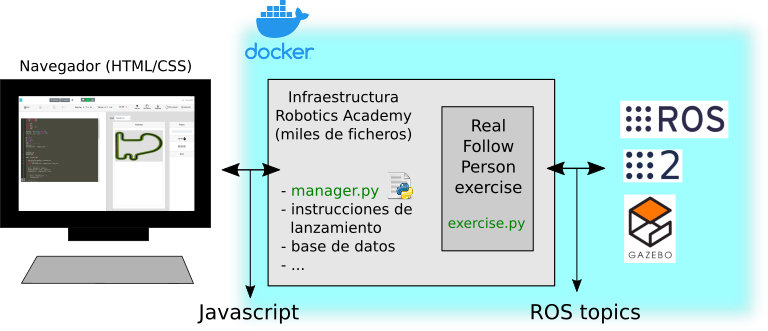
\includegraphics[width=15cm]{imagenes/esquema-robotics-academy.png}
  \end{center}
  \caption{Infraestructura Robotics Academy}
  \label{fig:infraestructura_robotics_academy}
\end{figure}\

Cuando el usuario lanza un contenedor, se ejecuta el fichero \textbf{manager.py}. Este fichero se encarga del control (puesta en marcha, cierre, eventos...) y lanzamiento de todos los recursos necesarios para los ejercicios. El \textbf{manager.py} se comunica con el \textbf{exercise.py} del ejercicio que esté usando el usuario. Este último fichero se encarga de la comunicación con la plantilla web (eventos de javascript) así como la incorporación de los módulos de programación (HAL y GUI) que internamente se comunican con los nodos de ROS
